\documentclass[a4paper]{article}
\usepackage{fancyhdr}
\usepackage[includeheadfoot,left=1in, right=0.5in, top=0.5in, bottom=0.5in]{geometry}
\usepackage{lastpage}
\usepackage{extramarks}
\usepackage[usenames,dvipsnames]{color}
\usepackage{graphicx}
\usepackage{listings}
\usepackage{courier}
\usepackage{tikz}
\usepackage{color}
\usepackage{float}
\usepackage{url}
\usepackage{subfigure}
\usepackage{varwidth}
\usepackage{caption}
\usepackage{multirow}
\usepackage[pdfborder={0 0 0}]{hyperref}
\usepackage[compact,small]{titlesec}
\usepackage{microtype}
\usepackage{verbatim}
\usepackage{booktabs}
\usepackage{indentfirst}
\usepackage{enumitem}
\usepackage{pdfpages}

\captionsetup[sub]{labelsep=newline}

% line spacing
\linespread{1.0}

% bold item
\let\origitem\item
\renewcommand{\item}{\normalfont\origitem}
\newcommand{\bolditem}{\small\bfseries\origitem}

% indent item
\newcommand{\indentitem}{\setlength\itemindent{24pt}}

\parskip = 0.5\baselineskip
\setlength{\belowcaptionskip}{-\baselineskip}

\captionsetup{font=scriptsize}
\captionsetup{labelfont=bf}

\pagestyle{fancy}
\rhead{Samir Silbak \& Manasa Kasula}
\lhead{EECE6080 - Project}
\rfoot{Page\ \thepage\ of \protect\pageref{LastPage}}
\cfoot{}
\renewcommand\headrulewidth{0.4pt}
\renewcommand\footrulewidth{0.4pt}

% make verbatim text small
\makeatletter
\g@addto@macro\@verbatim\small
\makeatother

\setlength\parindent{0pt} % Removes all indentation from paragraphs
%\setlength\parindent{24pt}

\definecolor{sh_comment}{rgb}{0.12, 0.38, 0.18 } %adjusted, in Eclipse: {0.25, 0.42, 0.30 } = #3F6A4D
\definecolor{sh_keyword}{rgb}{0.37, 0.08, 0.25}  % #5F1441
\definecolor{sh_string}{rgb}{0.06, 0.10, 0.98} % #101AF9

%\sectionfont{\centering}
\lstset{
    language=vhdl,
    xleftmargin=.25in,
    xrightmargin=.25in,
    numbers=left,
    numberstyle=\tiny,
    frame=tb,
    showstringspaces=false,
    captionpos=b,
    stringstyle=\color{sh_string},
    keywordstyle = \color{sh_keyword}\bfseries,
    commentstyle=\color{sh_comment}\itshape,
    basicstyle=\small\sffamily,
    %numbersep=-5pt,
    belowskip=\baselineskip,
    aboveskip=\baselineskip
}
\usepackage{authblk}

\title{
    \vspace{2in}
    \textbf{VLSI \\}
    \vspace{10pt}
    \textbf{PROGRAMMABLE BINARY TREE COMPUTATION\\}
    \vspace{10pt}
    \textbf{CHIP NAME: PBTCKS}
    \vspace{2in}
}

\author[1]{Samir Silbak}
\author[2]{Manasa Kasula}

\affil[1]{silbaksr@mail.uc.edu}
\affil[2]{kasulama@mail.uc.edu
    \vspace{10pt}
}
\affil[1]{(513) 207-0687}
\affil[2]{(847) 612-7364
    \vspace{2.0in}
}
\titleformat*{\section}{\large\normalfont}

\begin{document}

%\includepdf{}
\maketitle
\newpage
\parskip = 0.2\baselineskip
\newpage
\tableofcontents
\newpage
\listoffigures
\listoftables
\lstlistoflistings
\parskip = 0.5\baselineskip
\newpage

\section{\textbf{Pinout Diagram}}
    \begin{figure}[H]
        \centering
        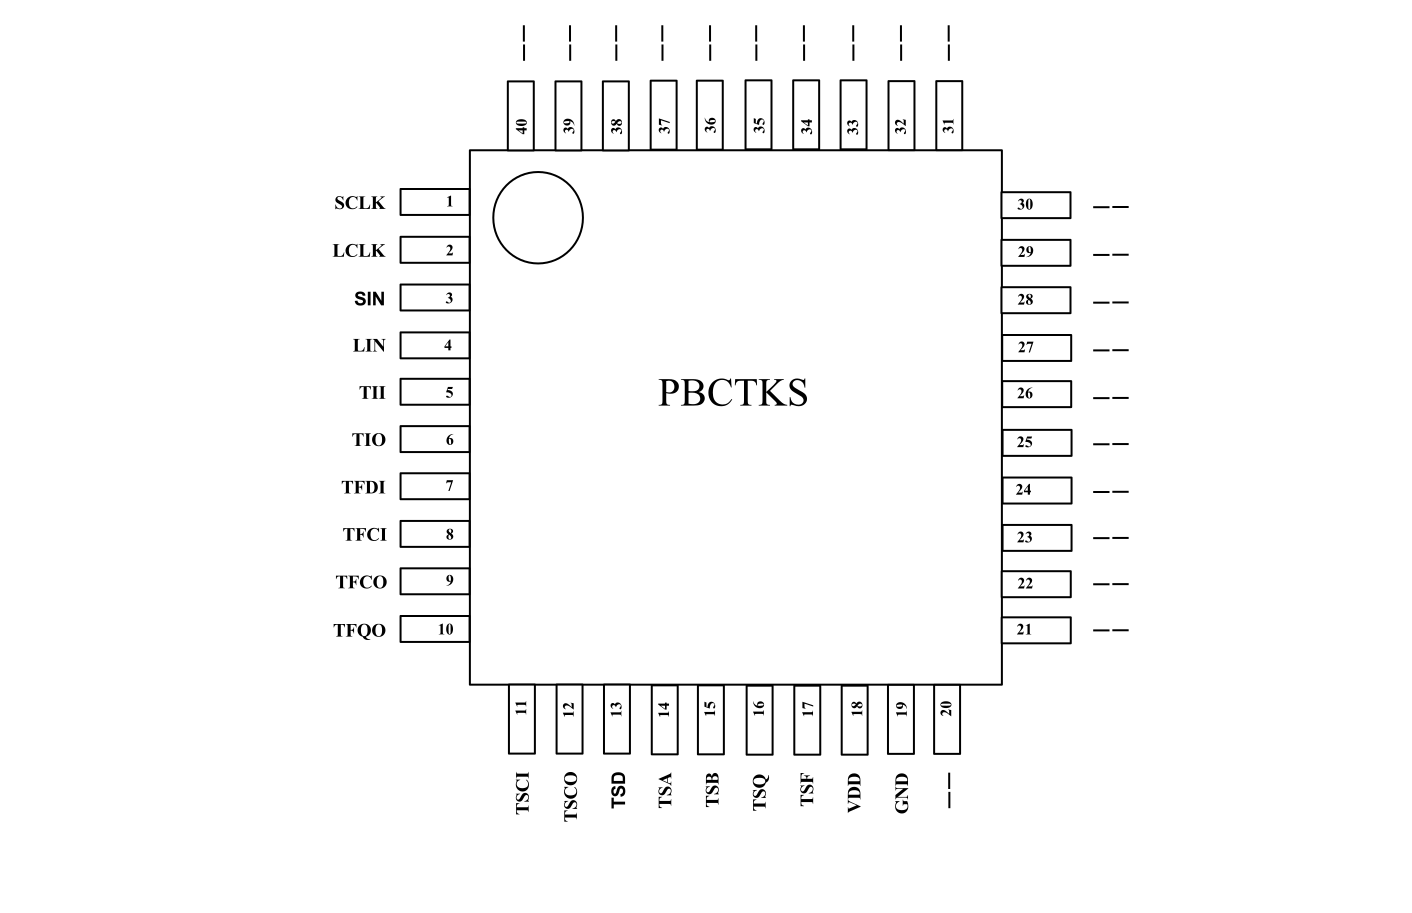
\includegraphics[width=\textwidth,height=\textheight,keepaspectratio]{../pinouts/pinout_diagram.png}
        \caption{\textbf{Pinout Diagram of the PBTCKS Chip}}
        \label{fig:gg}
    \end{figure}

\subsection{\textbf{Pinout Description}}
    \begin{table}[H]
        \centering
        \begin{tabular}{| l | l | c | p{10cm}|}
            \hline
            \textbf{Function}   & \textbf{Pin \#}       & \textbf{I/O}          &\textbf{Description}\\ \hline
            %\midrule
            %\midrule
                --              & 1                & --           & -- \\ \hline
                --              & 2                & --           & -- \\ \hline
                --              & 3                & --           & -- \\ \hline
                SCLKI           & 4                & I            & Shift Register Clock Input \\ \hline
                LCLKI           & 5                & I            & LUT Shift Register Clock Input \\ \hline
                SIN             & 6                & I            & Shift Register Input (P input) \\ \hline
                LIN             & 7                & I            & LUT Shift Register Input \\ \hline
                TMEI            & 8                & I            & Test Mode Enabled Input   \\ \hline
                --              & 9                & --           & -- \\ \hline
                --              & 10               & --           & -- \\ \hline

                TII             & 11               & I            & Test Inverter Input \\ \hline
                TIO             & 12               & O            & Test Inverter Output \\ \hline
                TFDI            & 13               & I            & Test Flip-Flop D Input \\ \hline
                TFCI            & 14               & I            & Test Flip-Flop Clock Input \\ \hline
                TFCO            & 15               & O            & Test Flip-Flop Clock Output \\ \hline
                TFQO            & 16               & O            & Test Flip-Flop Q Output \\ \hline
                --              & 17               & --           & -- \\ \hline
                --              & 18               & --           & -- \\ \hline
                --              & 19               & --           & -- \\ \hline
                GND             & 20               & --           & Ground Reference for I/O Pins \\ \hline

                --              & 21               & --           & -- \\ \hline
                --              & 22               & --           & -- \\ \hline
                TMEO            & 23               & O            & Test Mode Enabled Output \\ \hline
                LO              & 24               & O            & Shift Register Output of P input \\ \hline
                SO              & 25               & O            & Shift Register Output of LUT \\ \hline
                LCLKO           & 26               & O            & LUT Shift Register Clock Output \\ \hline
                SCLKO           & 27               & O            & Shift Register Clock Output \\ \hline
                F               & 28               & O            & Output of Computation of LUT \\ \hline
                --              & 29               & --           & -- \\ \hline
                --              & 30               & --           & -- \\ \hline

                VDD             & 31               & I            & Test LUT Slice B Input \\ \hline
                TPO             & 32               & O              & Test P Slice Output \\ \hline
                TPI             & 33                & I             & TesT P Slice Input \\ \hline
                TSF             & 34               & O            & Test LUT Slice Mux Output \\ \hline
                TSQ             & 35               & O            & Test LUT Slice Shift Register Output \\ \hline
                TSB             & 36               & I            & Test LUT Slice B Address Input \\ \hline
                TSA             & 37               & I            & Test LUT Slice A Address Input \\ \hline
                TSD             & 38               & I            & Test LUT Slice Shift Register Input \\ \hline
                TSCO            & 39               & O            & Test LUT Slice Clock Output \\ \hline
                TSCI            & 40               & I            & Test LUT SLice Clock Input \\ \hline
            %\bottomrule
        \end{tabular}
        \caption{\textbf{Pinout Description}}
    \end{table}

    \newpage

\section{\textbf{Explaination of Chip Function}}
    The main functionality of the chip is to be able to take N-bit inputs and compute the combinational logic among
    all N-bit inputs. Each node in the binary tree is what constitutes the combinational function of two inputs. Each
    node is described to be a 4-bit Look Up Table (LUT). The LUT has the function of any combinational function the
    user wants to perform. For example, for an AND gate, the user must shift in ``0001'' into the LUT. Each LUT of
    all the nodes together create the ``program'' which are all cascaded together to perform a shift register. The binary
    tree accepts the input P and produces only a single bit output O. For example, if the user has 8 different inputs, an
    example of the function can be described as so: (A or B) or (C or D) or (E or F) or (G or H). Here we can see that we
    have 8 different inputs performing 7 different functions (in this case each function is the same) and only one single
    output, O. P is defined to be twice the number of leaf nodes in the binary tree, and the input is shifted in serially
    using a shift register. In order to ``program'' the LUTs with the specific functions, these also must be shifted
    in serially using a shift register. Therefore, going back to the case where we have 8 different inputs and 7 different
    LUT, we can see that we will have to shift in 28 (7*4) bits into the LUT shift register. Each set of LUT outputs are connected
    to a 2:1 multiplexer to choose the output of the function. What this means is that the inputs can be thought of the
    address line into the LUT, what ever value happens to be stored is the result of that computation. For example, the figure
    below shows the truth table for an AND gate, we see inputs A and B, these are the address lines into the LUT. Therefore,
    we see that the output value of the LUT can only be 1 in the last row of the truth table, this method is very efficient
    and in fact this is how FPGAs work, they use LUT to perform these combinational functions.

    \begin{table}[H]
        \centering
        \begin{tabular}{ l l | l }
            \hline
            \textbf{A}  & \textbf{B}       & \textbf{F} \\ \hline
                0 & 0 & 0 \\ \hline
                0 & 1 & 0 \\ \hline
                1 & 0 & 0 \\ \hline
                1 & 1 & 1 \\ \hline
        \end{tabular}
        \caption{\textbf{AND Gate Truth Table}}
    \end{table}

\subsection{\textbf{Configuration of Chip}}

    \begin{figure}[H]
        \centering
        \includegraphics[width=\textwidth,height=\textheight,keepaspectratio]{../../docs/waveforms/lut_shift.png}
        \caption{\textbf{Cycle Timing Diagram for LUT Shift Register}}
        \label{fig:gg}
    \end{figure}

    Here we can see that the only thing the user needs to do is shift in the ``function'' wanted among the inputs. Since
    the data bits get loaded in from MSB to LSB, the user must input the function in revers order. For example, if we
    want to perform an AND operation, we have to feed the data bits in like so: 1000.

    \begin{figure}[H]
        \centering
        \includegraphics[width=\textwidth,height=\textheight,keepaspectratio]{../../docs/waveforms/p_shiftreg.png}
        \caption{\textbf{Cycle Timing Diagram for P Input Shift Register}}
        \label{fig:gg}
    \end{figure}

    As described from above the user has to just feed in input P, but in reverse order. Note that in test mode, the
    user has to just toggle the TMEI high.

    \newpage

\section{\textbf{Inclusion and Explanation of the Test Mode}}

    In order to enable the test mode, the user must set the TMEI pin high. In doing so, we will bypass the last output
    of P and feed it into the shift register input of the LUT. This will connect all the flip flops together, and we can
    perform our scan chain to make sure the inputs are being shifted the way they are supposed to be. We will be able
    to monitor the output on the TMEO pin. Since only one clock line is required, we bypass the LUT clock line by just
    hooking up the clock line of the P shift register. If test mode is disabled however, then the circuit will perform
    back to its original function.

\section{\textbf{Major Design Decisions}}

    The first thing that needed to be accomplished was to assemble the bit-slice design with minimal hardware and hardware
    that was supported by the library given to us. For example, our LUT bit slice uses three 2:1 Multiplexers, we could have
    used a 4:1 multiplexer, but having done so, our design would have been more complex when designing our Magic layouts.

    We also wanted to make sure that the wiring would not be too complex between each LUT slice. Since this is a binary
    tree computation, we made sure to hook up the hardware in that fashion as it made it much easier to visualize how
    this needed to be connected while keeping in mind that we must connect each one to achieve the desirable 50MHz clock
    frequency.

    \newpage

\section{\textbf{Block Diagrams}}

\subsection{\textbf{Top Level Diagram}}
    \begin{figure}[H]
        \centering
        \includegraphics[width=\textwidth,height=\textheight,keepaspectratio]{../../logisim/hierarchical_top.png}
        \caption{\textbf{Hierarchical Design in Logisim}}
        \label{fig:gg}
    \end{figure}

    \begin{figure}[H]
        \centering
        \includegraphics[width=\textwidth,height=\textheight,keepaspectratio]{../../logisim/top.png}
        \caption{\textbf{Top Level Diagram (8 Inputs, 28-bit slice)}}
        \label{fig:gg}
    \end{figure}

%\subsection{\textbf{Top Level Diagram: LUT Slice and Shift Slice}}
%    \begin{figure}[H]
%        \centering
%        \includegraphics[width=\textwidth,height=\textheight,keepaspectratio]{../../logisim/top_level.png}
%        \caption{\textbf{Top Level Diagram (8 Inputs, 28-bit slice)}}
%        \label{fig:gg}
%    \end{figure}

    We can see that the slice design of a shift register is just made up of D-flip flops as shown in the above
    top level diagram for input P. Here we can see that we have P being twice the leaf nodes (8) in this case
    and the LUTs are all cascaded together giving us a total vector of 28 bits wide.

\subsection{\textbf{Bit Slice Design Scheme}}
    \begin{figure}[H]
        \centering
        \includegraphics[width=\textwidth,height=\textheight,keepaspectratio]{../../logisim/slice.png}
        \caption{\textbf{LUT Slice in Logisim}}
        \label{fig:gg}
    \end{figure}

    Here we can see we have three 2:1 multiplexers, and 4 D-flip flops. We have the input of the LUT
    getting shifted through the d-flip flops. Each set of two outputs from the D-flip flops are connected
    to the inputs of the mux on select line A. Then the output from each mux will be fed into the final mux
    performing the computation on select line B.

\subsection{\textbf{Top Level Test Mode Diagram}}
    \begin{figure}[H]
        \centering
        \includegraphics[width=\textwidth,height=\textheight,keepaspectratio]{../../logisim/hierarchical_test_top.png}
        \caption{\textbf{Hierarchical Test Design in Logisim}}
        \label{fig:gg}
    \end{figure}

    \begin{figure}[H]
        \centering
        \includegraphics[width=\textwidth,height=\textheight,keepaspectratio]{../../logisim/top_test.png}
        \caption{\textbf{Top Level Test Mode Diagram (8 Inputs, 28-bit slice)}}
        \label{fig:gg}
    \end{figure}

    This test mode is configured with two 2:1 multiplexers. Each multiplexer will select the input line whether
    we are in test or normal mode. In test mode enabled, we see that we need to feed in the last output of the shift register
    into the input of L\_IN, where L\_IN is the input data into the LUT. Also, the clock used to shift the P data in,
    must now be the same clock input for the LUT. If test mode is disabled, we can see that the multiplexer will select
    the L\_IN to be the data configured by the user (not the data outputted from P).

    \newpage

\section{\textbf{VHDL Models with Test Mode}}

\subsection{\textbf{Top Level Module}}

    \lstinputlisting[caption=\textbf{Top Module}]{../../vhdl/top.vhd}
    \begin{figure}[H]
        \centering
        \includegraphics[width=\textwidth,height=\textheight,keepaspectratio]{../../docs/rtl_pics/top_rtl.png}
        \caption{\textbf{RTL Design of Top Level}}
        \label{fig:gg}
    \end{figure}

    \newpage

\subsection{\textbf{Slice Modules}}
\subsubsection{\textbf{LUT}}

    \lstinputlisting[caption=\textbf{Lookup Table Slice Module}]{../../vhdl/lut_slice.vhd}

    \begin{figure}[H]
        \centering
        \includegraphics[width=\textwidth,height=\textheight,keepaspectratio]{../../docs/rtl_pics/lut_slice_rtl.png}
        \caption{\textbf{RTL Design of LUT Slice}}
        \label{fig:gg}
    \end{figure}

\subsubsection{\textbf{Shift Register}}

    \lstinputlisting[caption=\textbf{Lookup Table Slice Module}]{../../vhdl/shift_slice.vhd}

    \begin{figure}[H]
        \centering
        \includegraphics[width=\textwidth,height=\textheight,keepaspectratio]{../../docs/rtl_pics/shift_slice_rtl.png}
        \caption{\textbf{RTL Design of Shift Register Slice}}
        \label{fig:gg}
    \end{figure}

\subsection{\textbf{Gates}}
\subsubsection{\textbf{D-Flip Flop}}

    \lstinputlisting[caption=\textbf{D-Flip Flop Module}]{../../vhdl/dffposx1.vhd}

\subsubsection{\textbf{2:1 Multiplexer}}

    \lstinputlisting[caption=\textbf{2:1 Multiplexer Module}]{../../vhdl/mux2x1.vhd}

\subsection{\textbf{VHDL Test Benches}}

    \lstinputlisting[caption=\textbf{LUT Slice Test Bench Module}]{../../vhdl/lut_slice_tb.vhd}
    \lstinputlisting[caption=\textbf{Top Level Test Bench Module}]{../../vhdl/top_tb.vhd}

\section{\textbf{VHDL Waveform Plots and Results}}

    \begin{figure}[H]
        \centering
        \includegraphics[width=\textwidth,height=\textheight,keepaspectratio]{../../vhdl/waveforms/andgate_lutslice.png}
        \caption{\textbf{AND Gate of LUT Slice}}
        \label{fig:gg}
    \end{figure}
    \begin{figure}[H]
        \centering
        \includegraphics[width=\textwidth,height=\textheight,keepaspectratio]{../../vhdl/waveforms/nandgate_lutslice.png}
        \caption{\textbf{NAND Gate of LUT Slice}}
        \label{fig:gg}
    \end{figure}
    \begin{figure}[H]
        \centering
        \includegraphics[width=\textwidth,height=\textheight,keepaspectratio]{../../vhdl/waveforms/orgate_lutslice.png}
        \caption{\textbf{OR Gate of LUT Slice}}
        \label{fig:gg}
    \end{figure}
    \begin{figure}[H]
        \centering
        \includegraphics[width=\textwidth,height=\textheight,keepaspectratio]{../../vhdl/waveforms/norgate_lutslice.png}
        \caption{\textbf{NOR Gate of LUT Slice}}
        \label{fig:gg}
    \end{figure}
    \begin{figure}[H]
        \centering
        \includegraphics[width=\textwidth,height=\textheight,keepaspectratio]{../../vhdl/waveforms/xorgate_lutslice.png}
        \caption{\textbf{XOR Gate of LUT Slice}}
        \label{fig:gg}
    \end{figure}

    Before we could go on with designing the top level in VHDL, we had to make sure that the slice itself worked first. Here
    we are just showing just a few waveforms from each function. As we can see here, each gate that was tested performed
    as expected.

    \begin{figure}[H]
        \centering
        \includegraphics[width=\textwidth,height=\textheight,keepaspectratio]{../../vhdl/waveforms/top_tb.png}
        \caption{\textbf{Waveform for Top Test Bench}}
        \label{fig:gg}
    \end{figure}

    Since we are testing with 8 input values, there are 2**28 combinations for the combinational functions. Since that is
    way more than we can test, we selected a few to test. We can see the results in the above waveform (Test Mode Disabled).

    \begin{figure}[H]
        \centering
        \includegraphics[width=\textwidth,height=\textheight,keepaspectratio]{../../vhdl/waveforms/top_test.png}
        \caption{\textbf{Waveform for Top Test Bench for Test Enabled}}
        \label{fig:gg}
    \end{figure}

    This is with Test Enabled for N=2. Here we can see the output of F at the very last clock cycle. In this case we
    tested the inputs 1111, and made sure our AND gate worked properly, and surely enough it works. We can see that F
    is high at the end of the simulation. We tested other functions and inputs as well, but we are just showing one waveform
    to keep things compact.

\section{\textbf{Work Division}}
    \begin{table}[H]
        \centering
        \begin{tabular}{l | p{8cm}}
            \hline
            \textbf{Student}   & \textbf{Task} \\ \hline
            \midrule
                Both        & Pin-out Diagram. \\
                Both        & Explanation of how the chip works. \\
                Both        & Description of the major design decisions made. \\
                Both        & Inclusion and explanation of the test mode. \\
                Silbak      & VHDL LUT slice Module \\
                Kasula      & VHDL LUT slice Test Bench Module \\
                Silbak      & VHDL Top Level Module \\
                Both        & VHDL Top Level Test Bench Module \\
                Silbak      & LUT Slice Block Diagram \\
                Kasula      & LUT Slice Top Level Diagram \\
        \end{tabular}
        \caption{\textbf{Task Assignment}}
    \end{table}
\end{document}
